\documentclass[12pt]{article}

\usepackage[margin=1in]{geometry}
\usepackage{amsfonts,amsmath,amssymb}
\usepackage{multicol}
\usepackage{graphicx}

\usepackage{float}
\usepackage[nottoc, notlot, notlof]{tocbibind}
\usepackage{hyperref}
\usepackage{enumitem}
\usepackage{caption}
\usepackage{subcaption}
\usepackage[T1]{fontenc}
%\usepackage[utf8]{inputenc}
\usepackage{xcolor}
\usepackage{pgfgantt}
\usepackage{rotating}
%\usepackage[graphicx]{realboxes}

\usepackage{color}
\definecolor{myblue}{rgb}{.8, .8, 1}
\definecolor{LightGray}{gray}{0.9}

\usepackage[most]{tcolorbox}
\tcbset{
	enhanced,
	colback=myblue!100!white,
	boxrule=0.1pt,
	colframe=myblue!100!black,
	fonttitle=\bfseries
}

\usepackage{minted} % For code 
\usepackage{tikz} % For checkmark



%\graphicspath{{/home/kushik/Kushik/VIT/Eighth semester/MagneticMirror/latex/forreport/Studies/}}

\def\checkmark{\tikz\fill[scale=0.5](0,.35) -- (.25,0) -- (1,.7) -- (.25,.15) -- cycle;} %define checkmark

\begin{document}
	
	\section{Study 2}
	
	Single particle \\
	Positions 
	\begin{figure}[H]
		\begin{multicols}{2}
			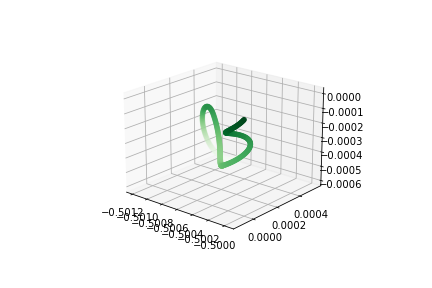
\includegraphics[width=\linewidth, height=6cm]{ps2.png} \caption{position} \label{ps2} \par
			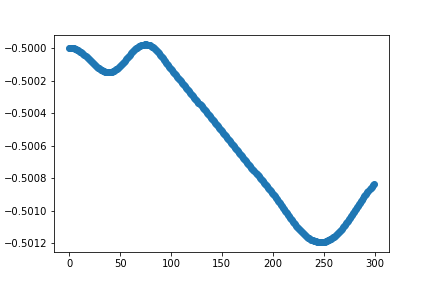
\includegraphics[width=\linewidth, height=6cm]{psx2.png} \caption{$x$-component of position} \label{psx2} \par
		\end{multicols}
	\end{figure}
	\begin{figure}[H]
		\begin{multicols}{2}
			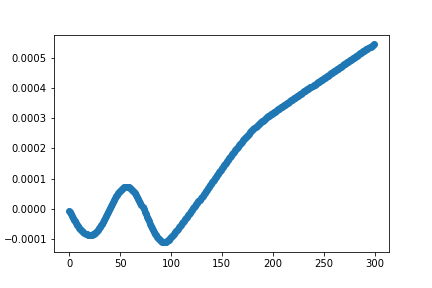
\includegraphics[width=\linewidth, height=6cm]{psy2.png} \caption{$y$-component of position} \label{psy2} \par
			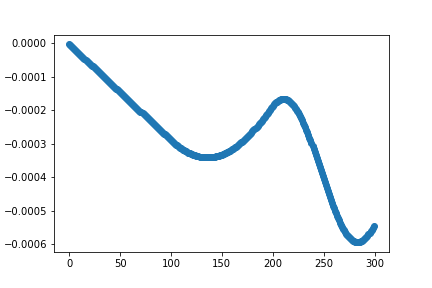
\includegraphics[width=\linewidth, height=6cm]{psz2.png} \caption{$z$-component of position} \label{psz2} \par
		\end{multicols}
	\end{figure}
	
	Velocity
	\begin{figure}[H]
		\begin{multicols}{2}
			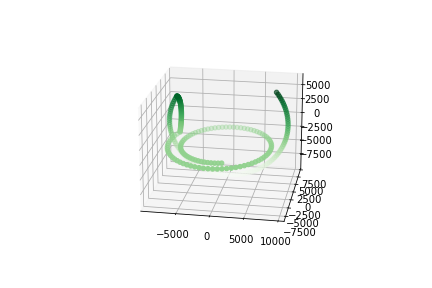
\includegraphics[width=\linewidth, height=6cm]{vs2.png} \caption{velocity} \label{vs2} \par
			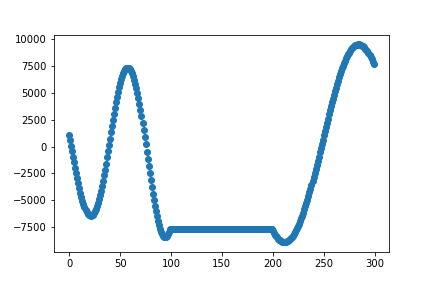
\includegraphics[width=\linewidth, height=6cm]{vsx2.png} \caption{$x$-component of velocity} \label{vsx2} \par
		\end{multicols}
	\end{figure}
	\begin{figure}[H]
		\begin{multicols}{2}
			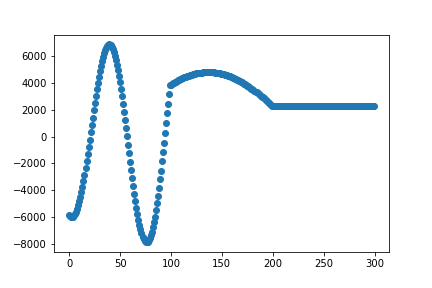
\includegraphics[width=\linewidth, height=6cm]{vsy2.png} \caption{$y$-component of velocity} \label{vsy2} \par
			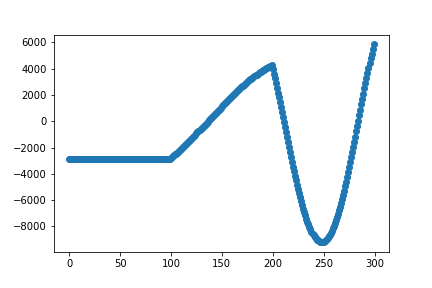
\includegraphics[width=\linewidth, height=6cm]{vsz2.png} \caption{$z$-component of velocity} \label{vsz2} \par
		\end{multicols}
	\end{figure}
	
	Multipartilces\\
	Positions
	\begin{figure}[H]
		\begin{multicols}{2}
			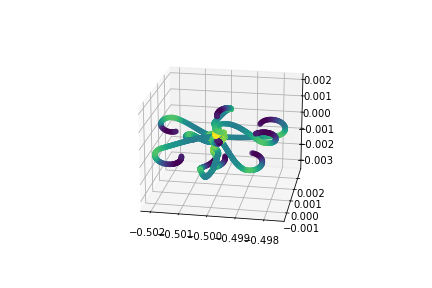
\includegraphics[width=\linewidth, height=6cm]{multips2.png} \caption{positions} \label{multips2} \par
			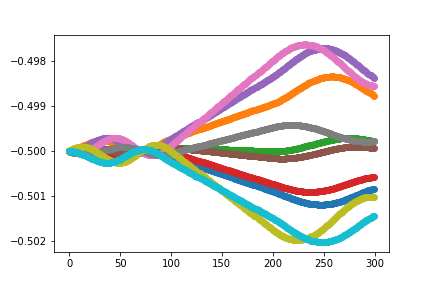
\includegraphics[width=\linewidth, height=6cm]{multipsx2.png} \caption{$x$-component of positions} \label{multipsx2} \par
		\end{multicols}
	\end{figure}
	\begin{figure}[H]
		\begin{multicols}{2}
			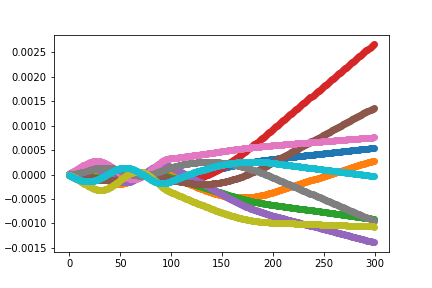
\includegraphics[width=\linewidth, height=6cm]{multipsy2.png} \caption{$y$-component of positions} \label{multipsy2} \par
			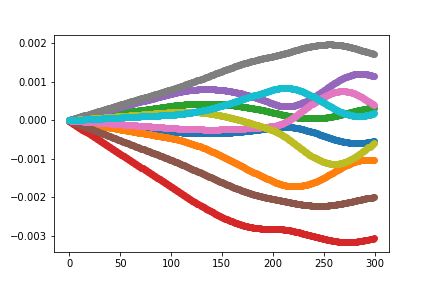
\includegraphics[width=\linewidth, height=6cm]{multipsz2.png} \caption{$z$-component of positions} \label{multipsz2} \par
		\end{multicols}
	\end{figure}

	Velocities
	\begin{figure}[H]
		\begin{multicols}{2}
			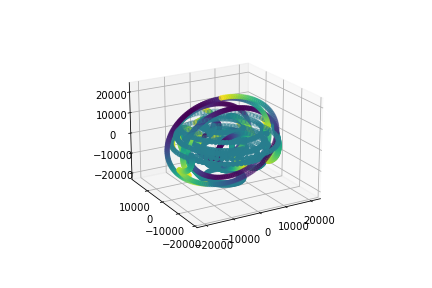
\includegraphics[width=\linewidth, height=6cm]{multivs2.png} \caption{velocities} \label{multivs2} \par
			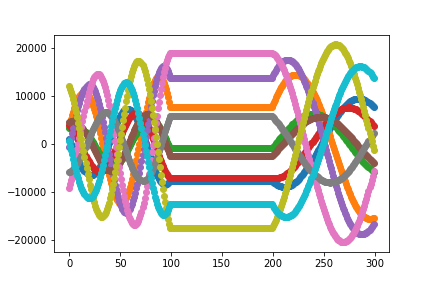
\includegraphics[width=\linewidth, height=6cm]{multivsx2.png} \caption{$x$-component of velocities} \label{multivsx2} \par
		\end{multicols}
	\end{figure}
	\begin{figure}[H]
		\begin{multicols}{2}
			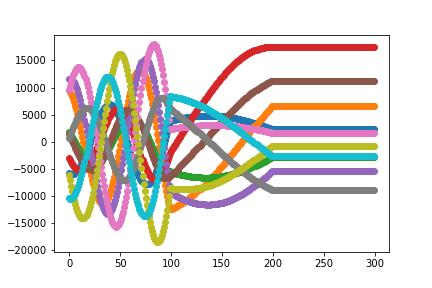
\includegraphics[width=\linewidth, height=6cm]{multivsy2.png} \caption{$y$-component of velocities} \label{multivsy2} \par
			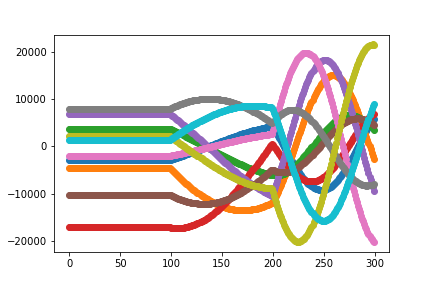
\includegraphics[width=\linewidth, height=6cm]{multivsz2.png} \caption{$z$-component of velocities} \label{multivsz2} \par
		\end{multicols}
	\end{figure}
	
	\section{Study 3}
	
	Single particle \\
	Positions 
	\begin{figure}[H]
		\begin{multicols}{2}
			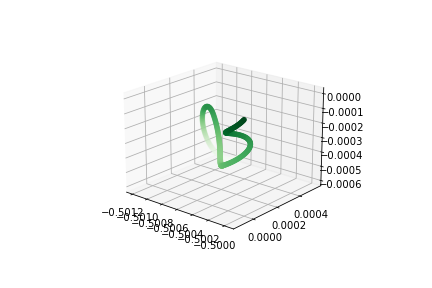
\includegraphics[width=\linewidth, height=6cm]{ps2.png} \caption{position} \label{ps2} \par
			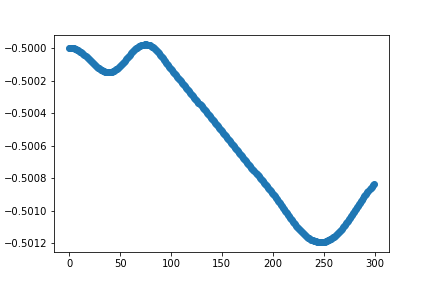
\includegraphics[width=\linewidth, height=6cm]{psx2.png} \caption{$x$-component of position} \label{psx2} \par
		\end{multicols}
	\end{figure}
	\begin{figure}[H]
		\begin{multicols}{2}
			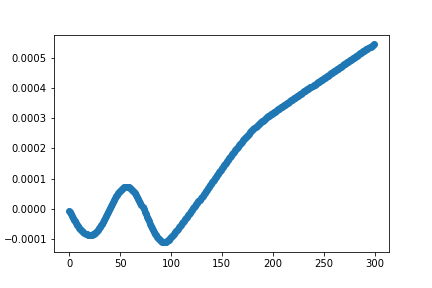
\includegraphics[width=\linewidth, height=6cm]{psy2.png} \caption{$y$-component of position} \label{psy2} \par
			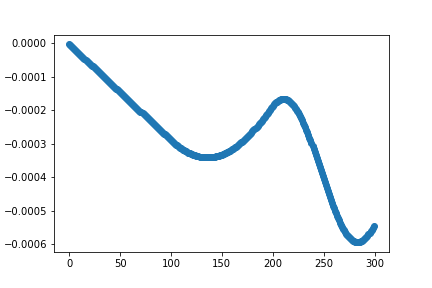
\includegraphics[width=\linewidth, height=6cm]{psz2.png} \caption{$z$-component of position} \label{psz2} \par
		\end{multicols}
	\end{figure}
	
	Velocity
	\begin{figure}[H]
		\begin{multicols}{2}
			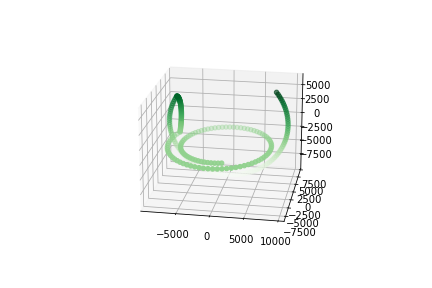
\includegraphics[width=\linewidth, height=6cm]{vs2.png} \caption{velocity} \label{vs2} \par
			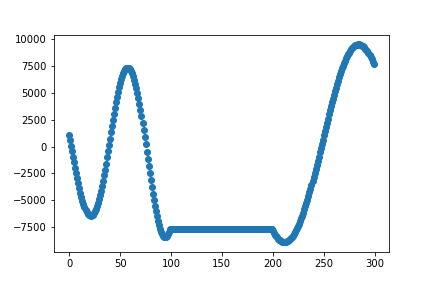
\includegraphics[width=\linewidth, height=6cm]{vsx2.png} \caption{$x$-component of velocity} \label{vsx2} \par
		\end{multicols}
	\end{figure}
	\begin{figure}[H]
		\begin{multicols}{2}
			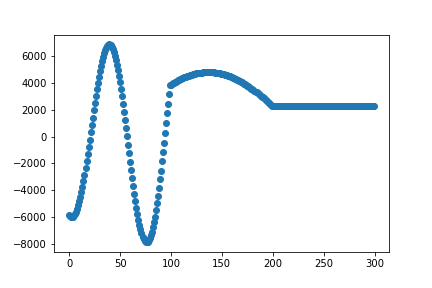
\includegraphics[width=\linewidth, height=6cm]{vsy2.png} \caption{$y$-component of velocity} \label{vsy2} \par
			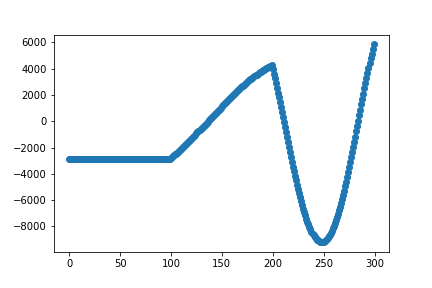
\includegraphics[width=\linewidth, height=6cm]{vsz2.png} \caption{$z$-component of velocity} \label{vsz2} \par
		\end{multicols}
	\end{figure}
	
	Multipartilces\\
	Positions
	\begin{figure}[H]
		\begin{multicols}{2}
			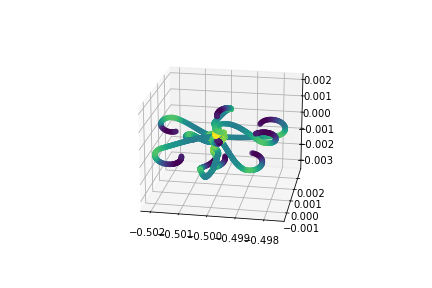
\includegraphics[width=\linewidth, height=6cm]{multips2.png} \caption{positions} \label{multips2} \par
			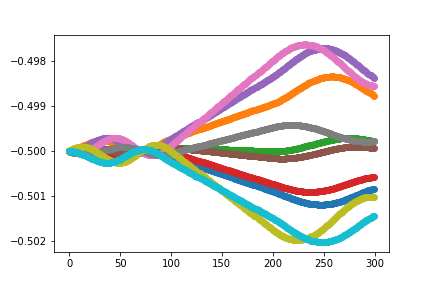
\includegraphics[width=\linewidth, height=6cm]{multipsx2.png} \caption{$x$-component of positions} \label{multipsx2} \par
		\end{multicols}
	\end{figure}
	\begin{figure}[H]
		\begin{multicols}{2}
			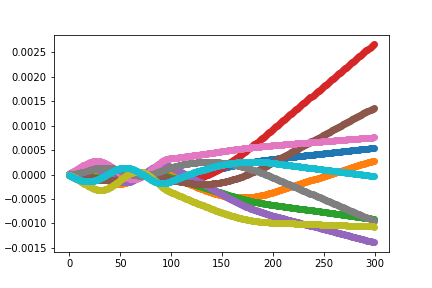
\includegraphics[width=\linewidth, height=6cm]{multipsy2.png} \caption{$y$-component of positions} \label{multipsy2} \par
			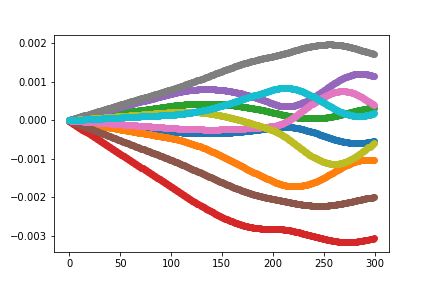
\includegraphics[width=\linewidth, height=6cm]{multipsz2.png} \caption{$z$-component of positions} \label{multipsz2} \par
		\end{multicols}
	\end{figure}
	
	Velocities
	\begin{figure}[H]
		\begin{multicols}{2}
			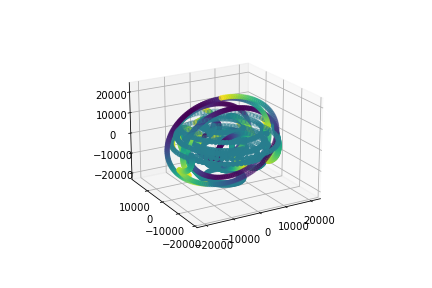
\includegraphics[width=\linewidth, height=6cm]{multivs2.png} \caption{velocities} \label{multivs2} \par
			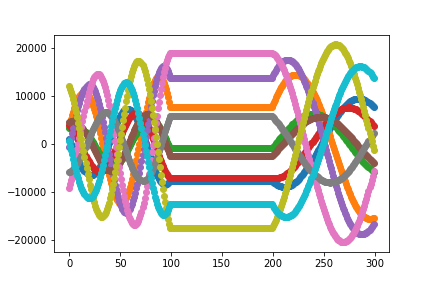
\includegraphics[width=\linewidth, height=6cm]{multivsx2.png} \caption{$x$-component of velocities} \label{multivsx2} \par
		\end{multicols}
	\end{figure}
	\begin{figure}[H]
		\begin{multicols}{2}
			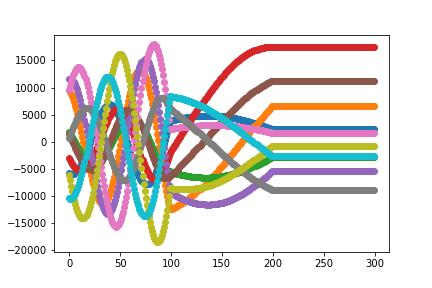
\includegraphics[width=\linewidth, height=6cm]{multivsy2.png} \caption{$y$-component of velocities} \label{multivsy2} \par
			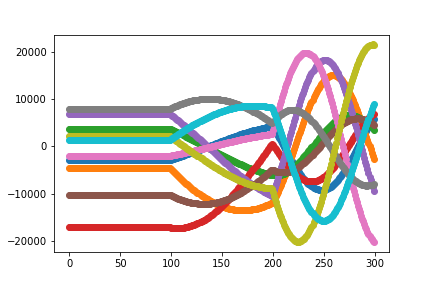
\includegraphics[width=\linewidth, height=6cm]{multivsz2.png} \caption{$z$-component of velocities} \label{multivsz2} \par
		\end{multicols}
	\end{figure}

\begin{thebibliography}{}
	\bibitem{blog} Florian LB (GitHub user). \textit{Charged Particle Trajectories in Electric and Magnetic Fields}. Thu, 28 Jan 2016. \textit{https://flothesof.github.io/charged-particle-trajectories-E-and-B-fields.html}
\end{thebibliography}
\end{document}